\section{An Overview}

\begin{frame}{Optimal Transport}
    \scriptsize
    \vspace{-1.5em}
    \begin{figure}
        \begin{minipage}[t]{0.6\linewidth}
            \vspace{0pt}
            \textbf{Core problem:} the distance between two probability measures.

            \textbf{First intruduced} in 1781 by Monge.

            \textbf{Relative subjects:} probability theory, geometry, graph theory, machine learning...

            \textbf{Applications:}
            \begin{itemize}
                \item Image registration and warping;
                \item Reflector design;
                \item Retrieving information from shadowgraphy and proton radiography;
                \item Seismic tomography and reflection seismology.
            \end{itemize}

            \textbf{Some well-known researchers:}
            \begin{itemize}
                \item Gasoard Monge (France);
                \item Leonid Kantorovich (Russia);
                \item Yann Brenier (France);
                \item Xianfeng Gu (顾险峰, China);
            \end{itemize}
        \end{minipage}
        \captionsetup{font=tiny}
        \begin{minipage}[t]{0.38\linewidth}
            \vspace{0pt}
            \centering
            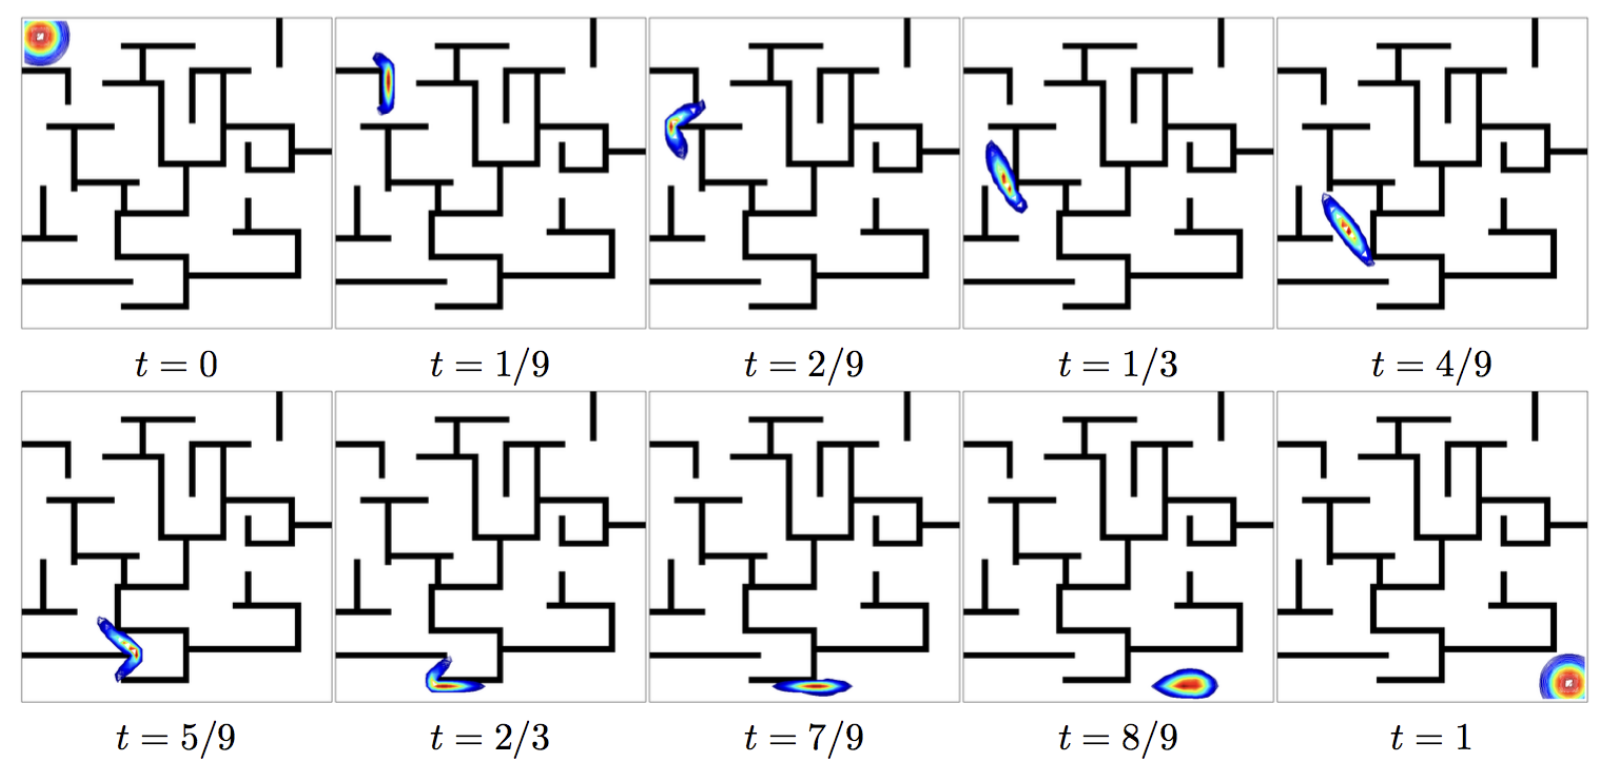
\includegraphics[width=0.9\textwidth]{png/maze.png}
            \caption{solving maze with OT}
            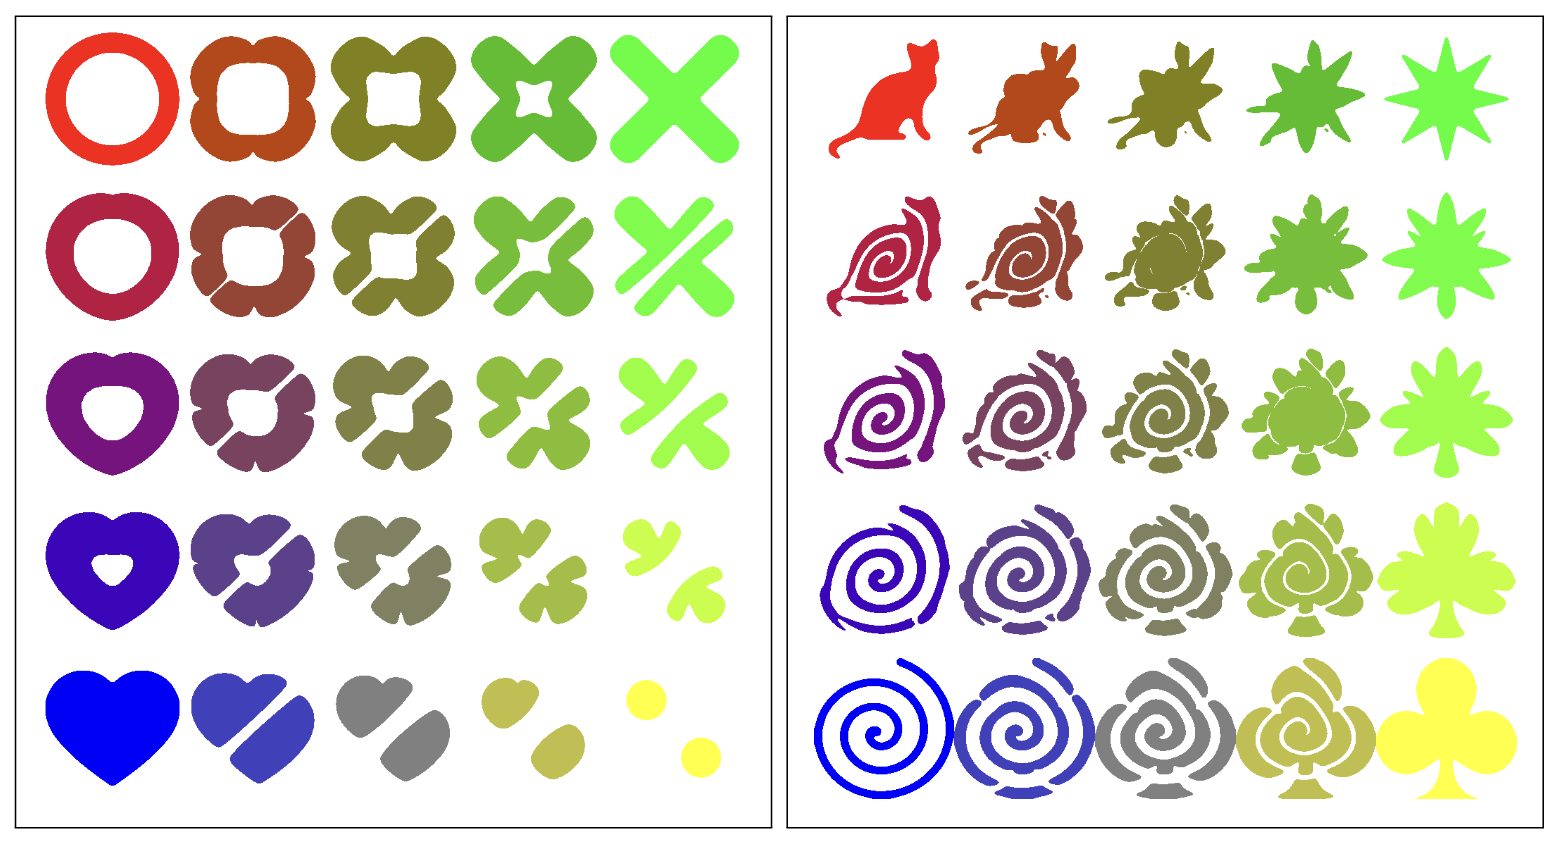
\includegraphics[width=0.9\textwidth]{png/2DShapeInterpolation.png}
            \caption{2D shape interpolation with OT}
        \end{minipage}
    \end{figure}

    \vspace{-1em}
    \begin{figure}
        \begin{minipage}[t]{0.48\textwidth}
            \vspace{0pt}
            \centering
            \captionsetup{font=tiny}
            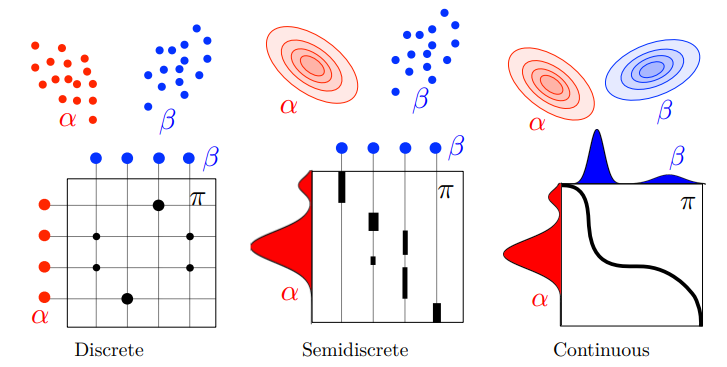
\includegraphics[width=0.7\textwidth]{png/3TypesOfOT.png}
            \vspace{-.7em}
            \caption{Three Types of OT}
        \end{minipage}
        \begin{minipage}[t]{0.5\textwidth}
            \vspace{0pt}
            \centering
            \captionsetup{font=tiny}
            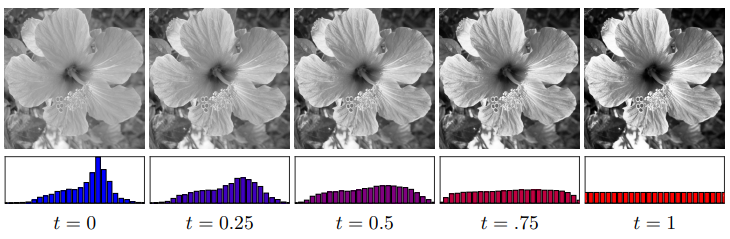
\includegraphics[width=0.8\textwidth]{png/HistogramEqualization.png}
            \vspace{-.7em}
            \caption{Histogram equalization with OT}
        \end{minipage}
    \end{figure}
\end{frame}